% *********************************************************************
% © 2021 Jeremy Sylvestre
%
% Permission is granted to copy, distribute and/or modify this document
% under the terms of the GNU Free Documentation License, Version 1.3 or
% any later version published by the Free Software Foundation; with no
% Invariant Sections, no Front-Cover Texts, and no Back-Cover Texts. A
% copy of the license is included in the appendix entitled “GNU Free
% Documentation License” that appears in the output document of this
% PreTeXt source code. All trademarks™ are the registered® marks of
% their respective owners.
%
% *********************************************************************

\newcommand*{\xmin}{-0.5}
\newcommand*{\xmax}{3.5}
\newcommand*{\ymin}{-0.5}
\newcommand*{\ymax}{3.5}

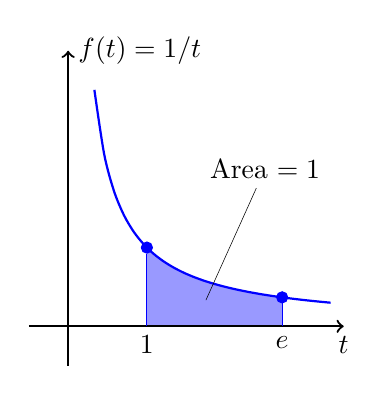
\begin{tikzpicture}
[
	closedpt/.style={circle,draw,fill,inner sep=0pt,minimum size=4pt},
	openpt/.style={circle,draw,inner sep=0pt,minimum size=4pt}
]

	% fills
	\fill[blue!40!white] (1,1) plot[domain=1:2.718] (\x,{1 / \x}) -- (2.718,0) -- (1,0) -- cycle;

	% axes
	\draw[->,thick] (\xmin,0) -- (\xmax,0) node[below] {$t$};
	\draw[->,thick] (0,\ymin) -- (0,\ymax) node[right] {$f(t) = 1/t$};

	% graph
	\draw[thick, blue, domain=0.333:3.333, smooth] plot (\x,{1 / \x});
	\node[blue,closedpt] at (1,1) (left) {};
	\draw[blue] (left) -- (1,0);
	\node[below] at (1,0) {$1$};
	\node[blue,closedpt] at (2.718,0.368) (right) {};
	\draw[blue] (right) -- (2.718,0);
	\node[below] at (2.718,0) {$e$};

	\node at (2.5,2) (int) {Area $= 1$};
	\draw[very thin] (int) -- (1.75,0.333);

\end{tikzpicture}
